\section{Continuous Random Variables}

\subsection{Features of Continuous Random Variables}

\begin{frame}{Continuous Random Variables}

\justifying
\structb{Definition.} Let $S$ be a sample space. A \highlightg{continuous random variable} is a map $X: S\rightarrow \R$ together with a function $f_X: \R\rightarrow \R$ with the properties that
\begin{enumerate}[(i).]
	\item $f_X(x) \geq 0$ for all $x\in \R$ and
	\item $\displaystyle \int_{-\infty}^{\infty} f_X(x) \U{d}x = 1.$
\end{enumerate}
The integral of $f_X$ is interpreted as the probability that $X$ assumes values $x$ in a given range, i.e.,
\begin{align*}
P[a\leq X \leq b] = \int_a^b f_X(x)\U{d}x.
\end{align*}
The function $f_X$ is called the \highlightg{probability density function} of random variable $X$.

\end{frame}

\begin{frame}{Cumulative Distribution}

\justifying
\structb{Definition.} Let $(X, f_X)$ be a continuous random variable. The cumulative distribution function for $X$ is defined by $F_X: \R\rightarrow \R$,
\begin{align*}
F_X(x) := P[X\leq x] = \int_{-\infty}^{x} f_X(y)\U{d}y.
\end{align*}
By the fundamental theorem of calculus, we can obtain the density function from $F_X$ by
\begin{align*}
f_X(x) = F_X'(x).
\end{align*}

\end{frame}


\begin{frame}{Expectation, Variance, and M.G.F.}

\justifying
\begin{itemize}
	\item \underline{Expectation}.
	\begin{align*}
	\U{E}[X] := \int_{\R} x\cdot f_X(x)\U{d}x.
	\end{align*}
	\item \underline{Variance}.
	\begin{align*}
	\U{Var}[X] := \U{E}[(X-\U{E}[X])^2] = \U{E}[X^2] - \U{E}[X]^2.
	\end{align*}
	\item \underline{Moment-generating function}.
	\begin{align*}
	m_X(t) = \U{E}[e^{tX}] = \int_{-\infty}^{\infty} e^{tx}f_X(x) \U{d}x.
	\end{align*}
\end{itemize}
\highlightr{Note.} All previous properties about expectation, variance and M.G.F. hold for continuous random variables.

\end{frame}


\begin{frame}{Location of Continuous Distributions}

\structb{Definitions.}
\begin{itemize}
	\justifying
	\item The \highlightg{median} $M_X$ is defined by $P[X\leq M_X] = 0.5$.
	\item The \highlightg{mean} is given by $\U{E}[X]$.
	\item The \highlightg{mode} $x_0$, is the location of the maximum of $f_X$.
\end{itemize}

\end{frame}


\subsection{Transformation of Random Variables}

\begin{frame}{Transformation of Random Variables}

\justifying
\structb{Theorem.} Let $X$ be a continuous random variable with density $f_X$. Let $Y = \varphi\circ X$, where $\varphi: \R\rightarrow \R$ is strictly monotonic and differentiable. The density for $Y$ is then given by
\begin{align*}
f_Y(y) = f_X(\varphi^{-1}(y))\cdot \left|\frac{\U{d}\varphi^{-1}(y)}{\U{d}y} \right|, \qquad \U{for\ } y\in \U{ran\ }\varphi
\end{align*}
and 
\begin{align*}
f_Y(y) = 0, \qquad \U{for\ } y\notin \U{ran\ } \varphi.
\end{align*}


\end{frame}


\begin{frame}{Transformation of Random Variables}

\justifying
\structb{Example 1.} A model for populations of microscopic organisms is exponential growth. Initially, $v$ organisms are introduced into a large tank of water, and let $X$ be the rate of growth. After time $t$, the population becomes $Y = ve^{Xt}$. Suppose $X$ is unknown and has a continuous distribution
\begin{align*}
f_X(x) = \left\{
\begin{array}{ll}
3(1-x)^2 & \U{for\ } 0 < x < 1, \\
0, & \U{otherwise}.
\end{array}
\right.
\end{align*}
What is the distribution of $Y$? \\
\only<2>{
	\structb{Solution.} \begin{enumerate}[(i).]
		\item Identify and calculate $\varphi^{-1}$ and $\dfrac{\U{d}\varphi^{-1}(y)}{\U{d}y}$.
		\item Substitute  $x$ with $\varphi^{-1}(y)$ in the density function of $X$.
	\end{enumerate}
}
\only<3>{
	\structb{Solution.} We have $\varphi(x) = ve^{xt}$, and thus
	\begin{align*}
	\varphi^{-1}(y) = \frac{1}{t}\log\left(\frac{y}{v} \right), \qquad \frac{\U{d}\varphi^{-1}(y)}{\U{d}y} = \frac{1}{ty}.
	\end{align*}
}
\uncover<4>{
	\structb{Solution (continued).} Therefore,
	\begin{align*}
	f_Y(y) = \left\{
	\begin{array}{ll}
	3\left(1 - \dfrac{1}{t}\log\left(\dfrac{y}{v} \right) \right)^2\cdot \dfrac{1}{ty}, & v < y < ve^t, \\
	0 & \U{otherwise}.
	\end{array}
	\right.
	\end{align*}
}


\end{frame}


\section{Common Distributions}

\subsection{Exponential Distribution}

\begin{frame}{Exponential Distribution}

\justifying
\structb{Definition.} A continuous random variable $(X, f_{\beta})$ a \highlightg{exponential distribution} with parameter $\beta$ if the probability density function is defined by
\begin{align*}
f_{\beta}(X) = \left\{
\begin{array}{ll}
\beta e^{-\beta x}, & x > 0, \\
0, & x\leq 0.
\end{array}
\right.
\end{align*}
\structb{Interpretation.} The time between successive arrivals of a Poisson process with rate $\lambda$ follows exponential distribution with parameter $\beta = \lambda$. (Recall $P[T > t] = e^{-\beta t}$.)\\
\highlightr{Note.} Memoryless property:
\begin{align*}
P[X > x + s|X > x] = P[X > s].
\end{align*}


\end{frame}

\begin{frame}{Exponential Distribution}

\justifying
\structb{Mean, variance and M.G.F.} 
\begin{itemize}
	\justifying
	\item \underline{Mean}. 
	\begin{align*}
	\U{E}[X] = \frac{1}{\beta}.
	\end{align*}
	\item \underline{Variance}.
	\begin{align*}
	\U{Var}[X] = \frac{1}{\beta^2}.
	\end{align*}
	\item \underline{M.G.F.}
	\begin{align*}
	m_X: (-\infty, \beta) \rightarrow \R, \qquad m_X(t) = \frac{1}{1-t/\beta}.
	\end{align*}
\end{itemize}

\end{frame}

\begin{frame}{Exponential Distribution}

\structb{Plots.}
\begin{figure}[htbp]
	\centering
	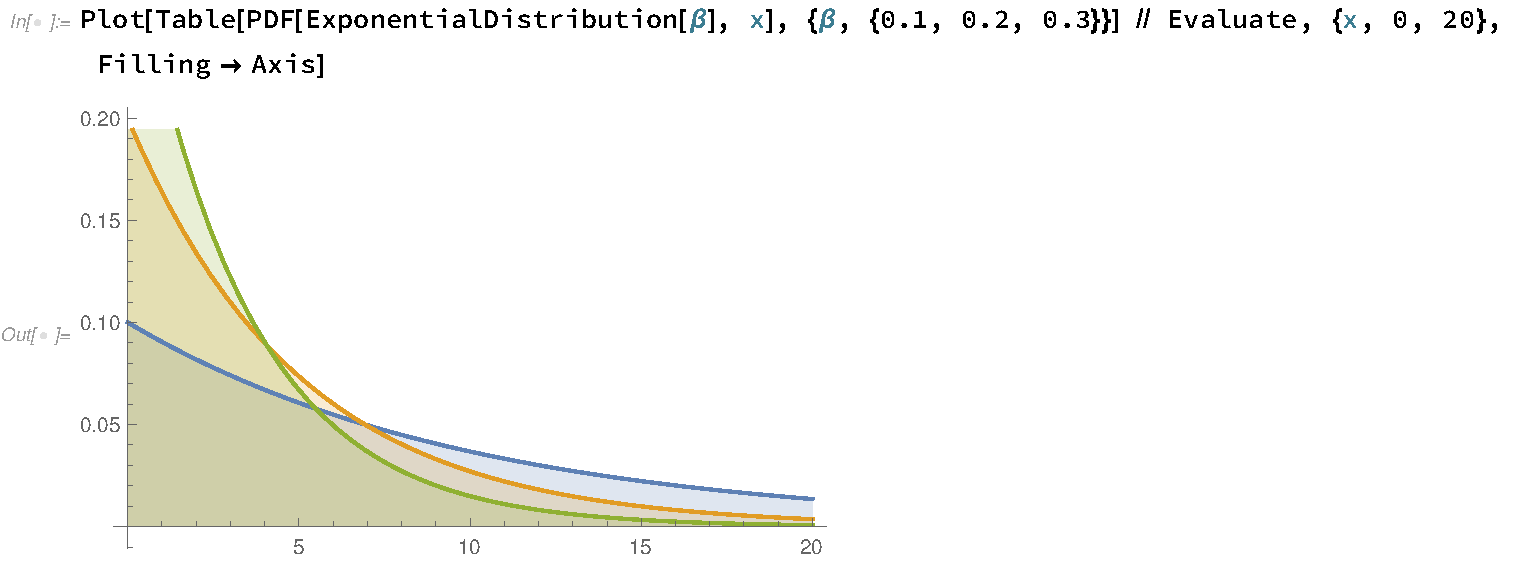
\includegraphics[width=\linewidth]{./images/rc2fig2.pdf}
\end{figure}

\end{frame}


\begin{frame}{Exponential Distribution}

\justifying
\structb{Example 2.} $n$ light bulbs are burning simultaneously and independently, and the lifetime for each bulb follows the $\U{Exp}(\beta)$. 
\begin{enumerate}[(i).]
	\justifying
	\item What is the distribution of the length of time $Y_1$ until the first failure in one of the $n$ bulbs?
	\item What is the distribution of the length of time $Y_2$ after the first failure until a second bulb fails?
\end{enumerate}
\uncover<2>{
	\structb{Solution (i).} Suppose random variables $X_1, \ldots, X_n$ satisfies that $X_i\sim \U{Exp}(\beta)$, and $Y_1 = \min\{X_1, \ldots, X_n\}$. Then for any $t > 0$,
	\begin{align*}
	P[Y_1 > t] & = P[X_1 > t, \ldots, X_n > t] \\
	& = P[X_1 > t]\times \cdots \times P[X_n > t] \\
	& = e^{-n\beta t},
	\end{align*}
	indicating an exponential distribution with parameter $n\beta$. What about (ii)?
}

\end{frame}


\subsection{Gamma Distribution}

\begin{frame}{Gamma Distribution}

\structb{Definition.} Let $\alpha, \beta \in \R, \alpha, \beta > 0$. A continuous random variable $(X, f_{\alpha, \beta})$ follows a \highlightg{gamma distribution} with parameters $\alpha$ and $\beta$ if the probability density function is given by
\begin{align*}
f_{\alpha, \beta}(x) = \left\{
\begin{array}{ll}
\dfrac{\beta^{\alpha}}{\Gamma(\alpha)} x^{\alpha-1} e^{-\beta x}, & x > 0, \\
0, & x \leq 0.
\end{array}
\right.
\end{align*}
where $\displaystyle\Gamma(\alpha) = \int_0^{\infty} z^{\alpha-1} e^{-z}\U{d}z, \alpha > 0$ is the Euler gamma function. \\
~\\
\structb{Interpretation.} The time needed for the next $r$ arrivals in a Poisson process with rate $\lambda$ follows a Gamma distribution with parameters $\alpha = r, \beta = \lambda$.

\end{frame}


\begin{frame}{Gamma Distribution}

\justifying
\structb{Mean, variance and M.G.F.} 
\begin{itemize}
	\justifying
	\item \underline{Mean}. 
	\begin{align*}
	\U{E}[X] = \frac{\alpha}{\beta}.
	\end{align*}
	\item \underline{Variance}.
	\begin{align*}
	\U{Var}[X] = \frac{\alpha}{\beta^2}.
	\end{align*}
	\item \underline{M.G.F.}
	\begin{align*}
	m_X: (-\infty, \beta) \rightarrow \R, \qquad m_X(t) = \frac{1}{(1-t/\beta)^{\alpha}}.
	\end{align*}
\end{itemize}

\end{frame}

\begin{frame}{Gamma Distribution}

\structb{Plots.}
\begin{figure}[htbp]
	\centering
	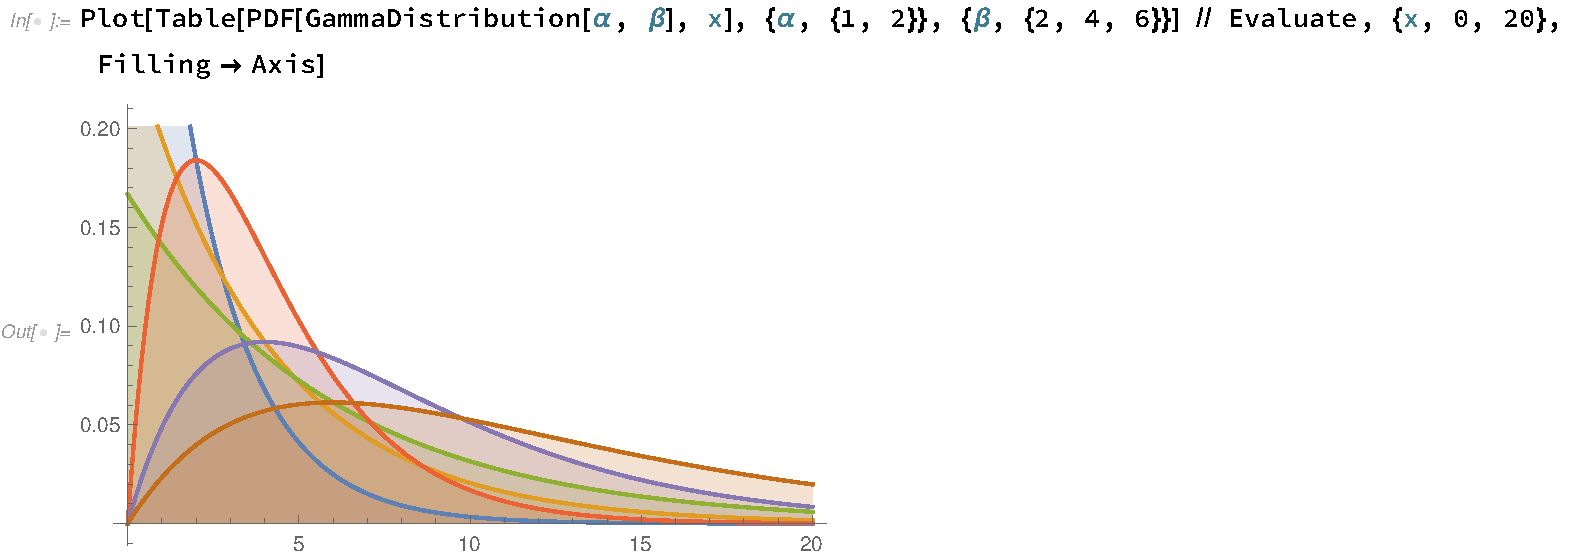
\includegraphics[width=\linewidth]{./images/rc2fig3.pdf}
\end{figure}

\end{frame}

\begin{frame}{Chi-Squared Distribution}

\justifying
\structb{Definition.} Let $\gamma\in \N$. A continuous random variable $(X_{\gamma}^2, f_X)$ follows a \highlightg{chi-squared distribution} with $\gamma$ degrees of freedom if the probability density function is given by
\begin{align*}
f_{\gamma}(x) = \left\{
\begin{array}{ll}
\dfrac{1}{2^{\gamma/2}\Gamma(\gamma/2)} x^{\gamma/2-1} e^{-x/2}, & x > 0, \\
0, & x\leq 0,
\end{array}
\right.
\end{align*}
which is a gamma distribution with $\alpha = \gamma/2, \beta = 1/2$. Therefore,
\begin{align*}
\U{E}[X^2_{\gamma}] = \gamma, \qquad \U{Var}[X_{\gamma}^2] = 2\gamma.
\end{align*}


\end{frame}


\begin{frame}{Chi-Squared Distribution}

\structb{Plots.}
\begin{figure}[htbp]
	\centering
	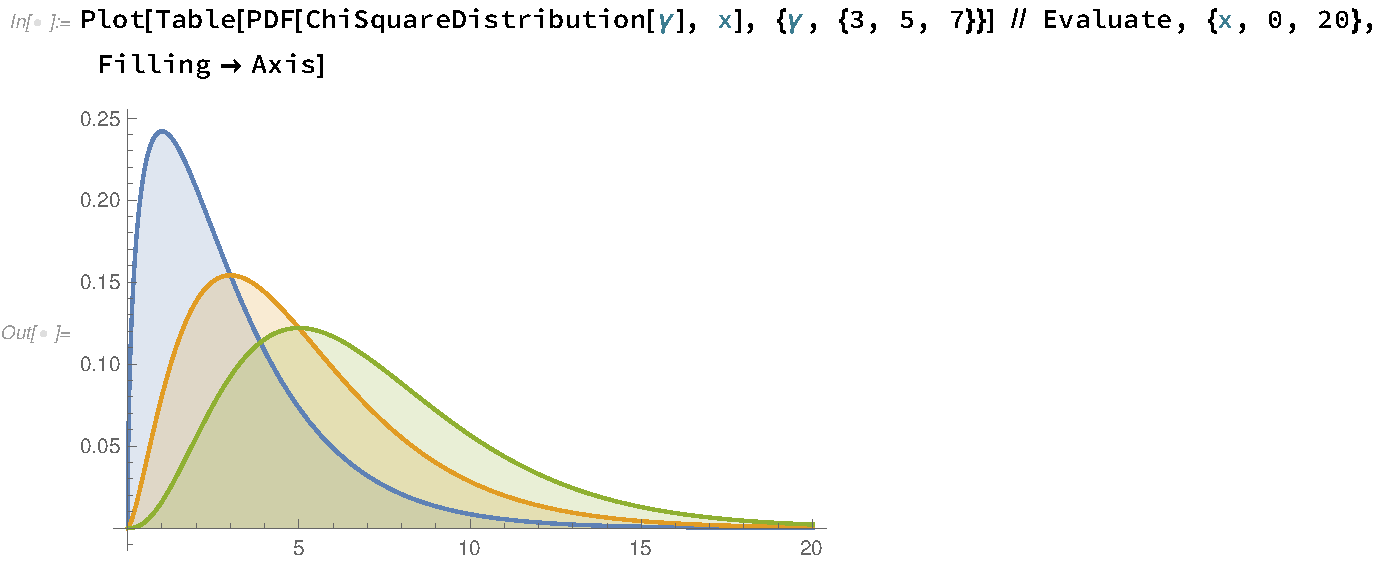
\includegraphics[width=\linewidth]{./images/rc2fig4.pdf}
\end{figure}

\end{frame}


\subsection{Normal Distribution}

\begin{frame}{Normal Distribution}

\justifying
\structb{Definition.} A continuous random variable $(X, f_{\mu, \sigma^2})$ has the \highlightg{normal distribution} with mean $\mu \in \R$ and variance $\sigma^2, \sigma > 0$ if the probability density function is given by
\begin{align*}
f_{\mu, \sigma^2} = \frac{1}{\sqrt{2\pi \sigma^2}} \exp\left[-\frac{1}{2}\left(\frac{x-\mu}{\sigma} \right)^2 \right], \qquad x\in \R.
\end{align*}

\end{frame}

\begin{frame}{Normal Distribution}

\justifying
\structb{Mean, variance and M.G.F.} 
\begin{itemize}
	\justifying
	\item \underline{Mean}. 
	\begin{align*}
	\U{E}[X] = \mu.
	\end{align*}
	\item \underline{Variance}.
	\begin{align*}
	\U{Var}[X] = \sigma^2.
	\end{align*}
	\item \underline{M.G.F.}
	\begin{align*}
	m_X: \R \rightarrow \R, \qquad m_X(t) = \exp\left(\mu t + \frac{1}{2}\sigma^2t^2 \right).
	\end{align*}
\end{itemize}

\end{frame}

\begin{frame}{Normal Distribution}

\structb{Plots.}
\begin{figure}[htbp]
	\centering
	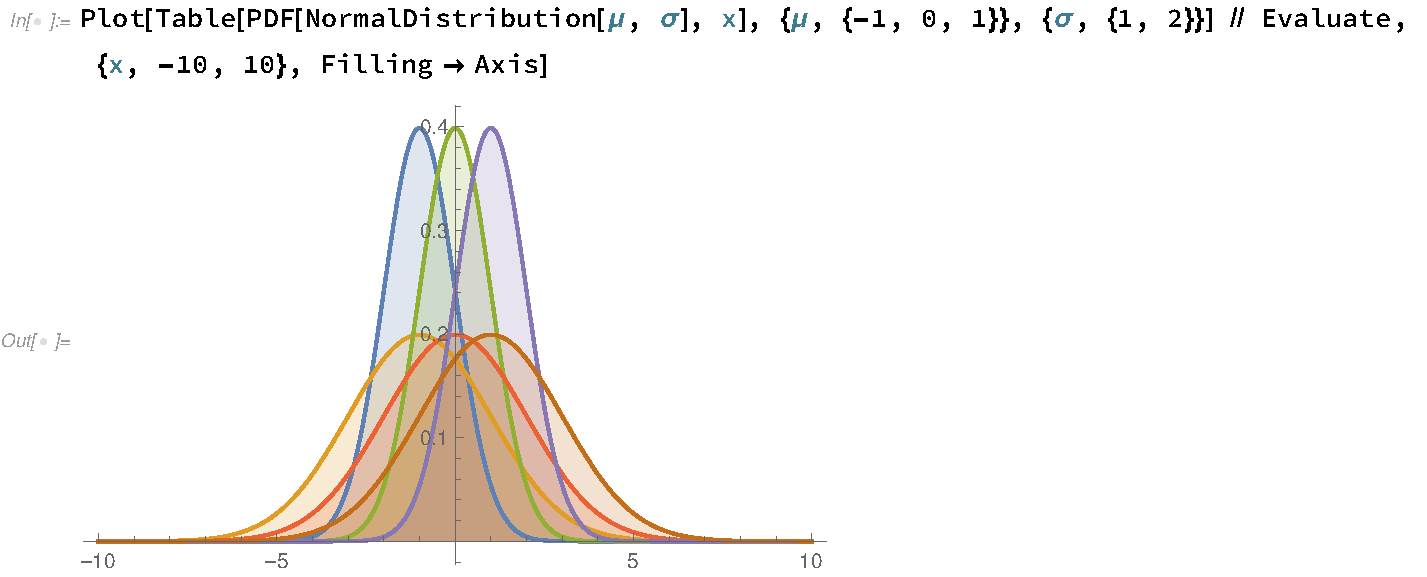
\includegraphics[width=\linewidth]{./images/rc2fig5.pdf}
\end{figure}

\end{frame}

\begin{frame}{Standardizing Normal Distribution}

\justifying
Suppose $X\sim \U{Normal}(\mu, \sigma^2)$. Then 
\begin{align*}
Z = \frac{X-\mu}{\sigma} \sim \U{Normal}(0, 1),
\end{align*}
where the normal distribution with mean $\mu$ and variance $\sigma^2$ is the \highlightg{standard normal distribution}. Furthermore, the cumulative distri-\\bution function of $X$ is given by
\begin{align*}
F(x) = \Phi\left(\frac{x-\mu}{\sigma} \right), \quad F^{-1}(p) = \mu + \sigma \Phi^{-1}(p),
\end{align*}
where $\Phi$ is the cumulative distribution function for the standard normal distribution function.

\end{frame}


\subsection{Connections of Distributions}

\begin{frame}{Distributions based on of Poisson Process}

\begin{figure}[htbp]
	\centering
	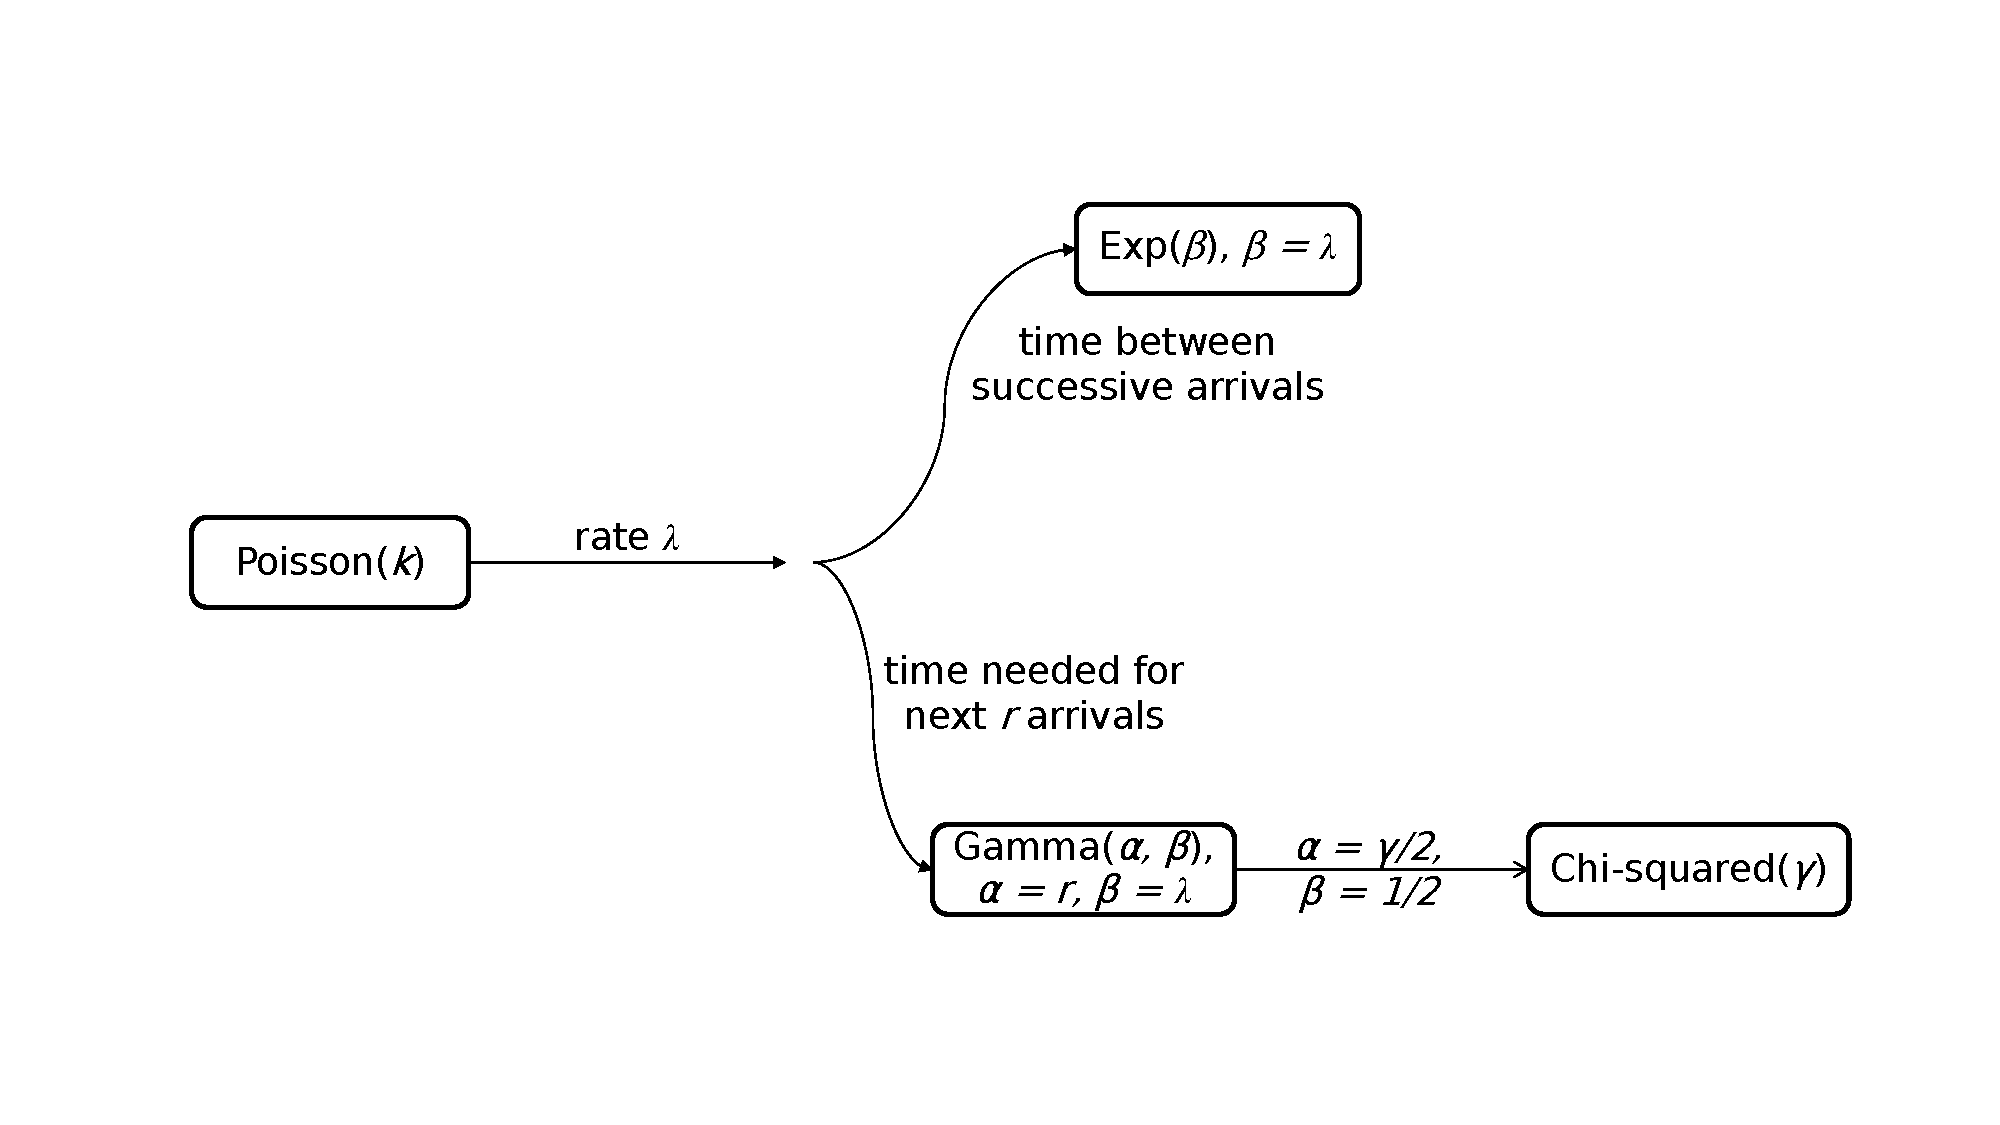
\includegraphics[width=11cm]{./images/rc2fig6.pdf}
	\caption{Connections of distributions based on Poisson process.}
\end{figure}

\end{frame}


\begin{frame}{Poisson, Gamma and Negative Binomial Distribution}

\structb{Application.} 
\begin{itemize}
	\justifying
	\item To ensure stability of an aircraft, the broken components should be removed, replaced, and repaired immediately
	\item When the components are repaired, the replacing component is removed from the aircraft and restored to storage.
	\item Suppose the components are returned in the same order as they are removed from the aircraft.
	\item \emph{Q}: How many components should be stored in case of such usage?
\end{itemize}


\end{frame}


\begin{frame}{Poisson, Gamma and Negative Binomial Distribution}

\structb{Application (continued).} 
\begin{figure}[htbp]
	\centering
	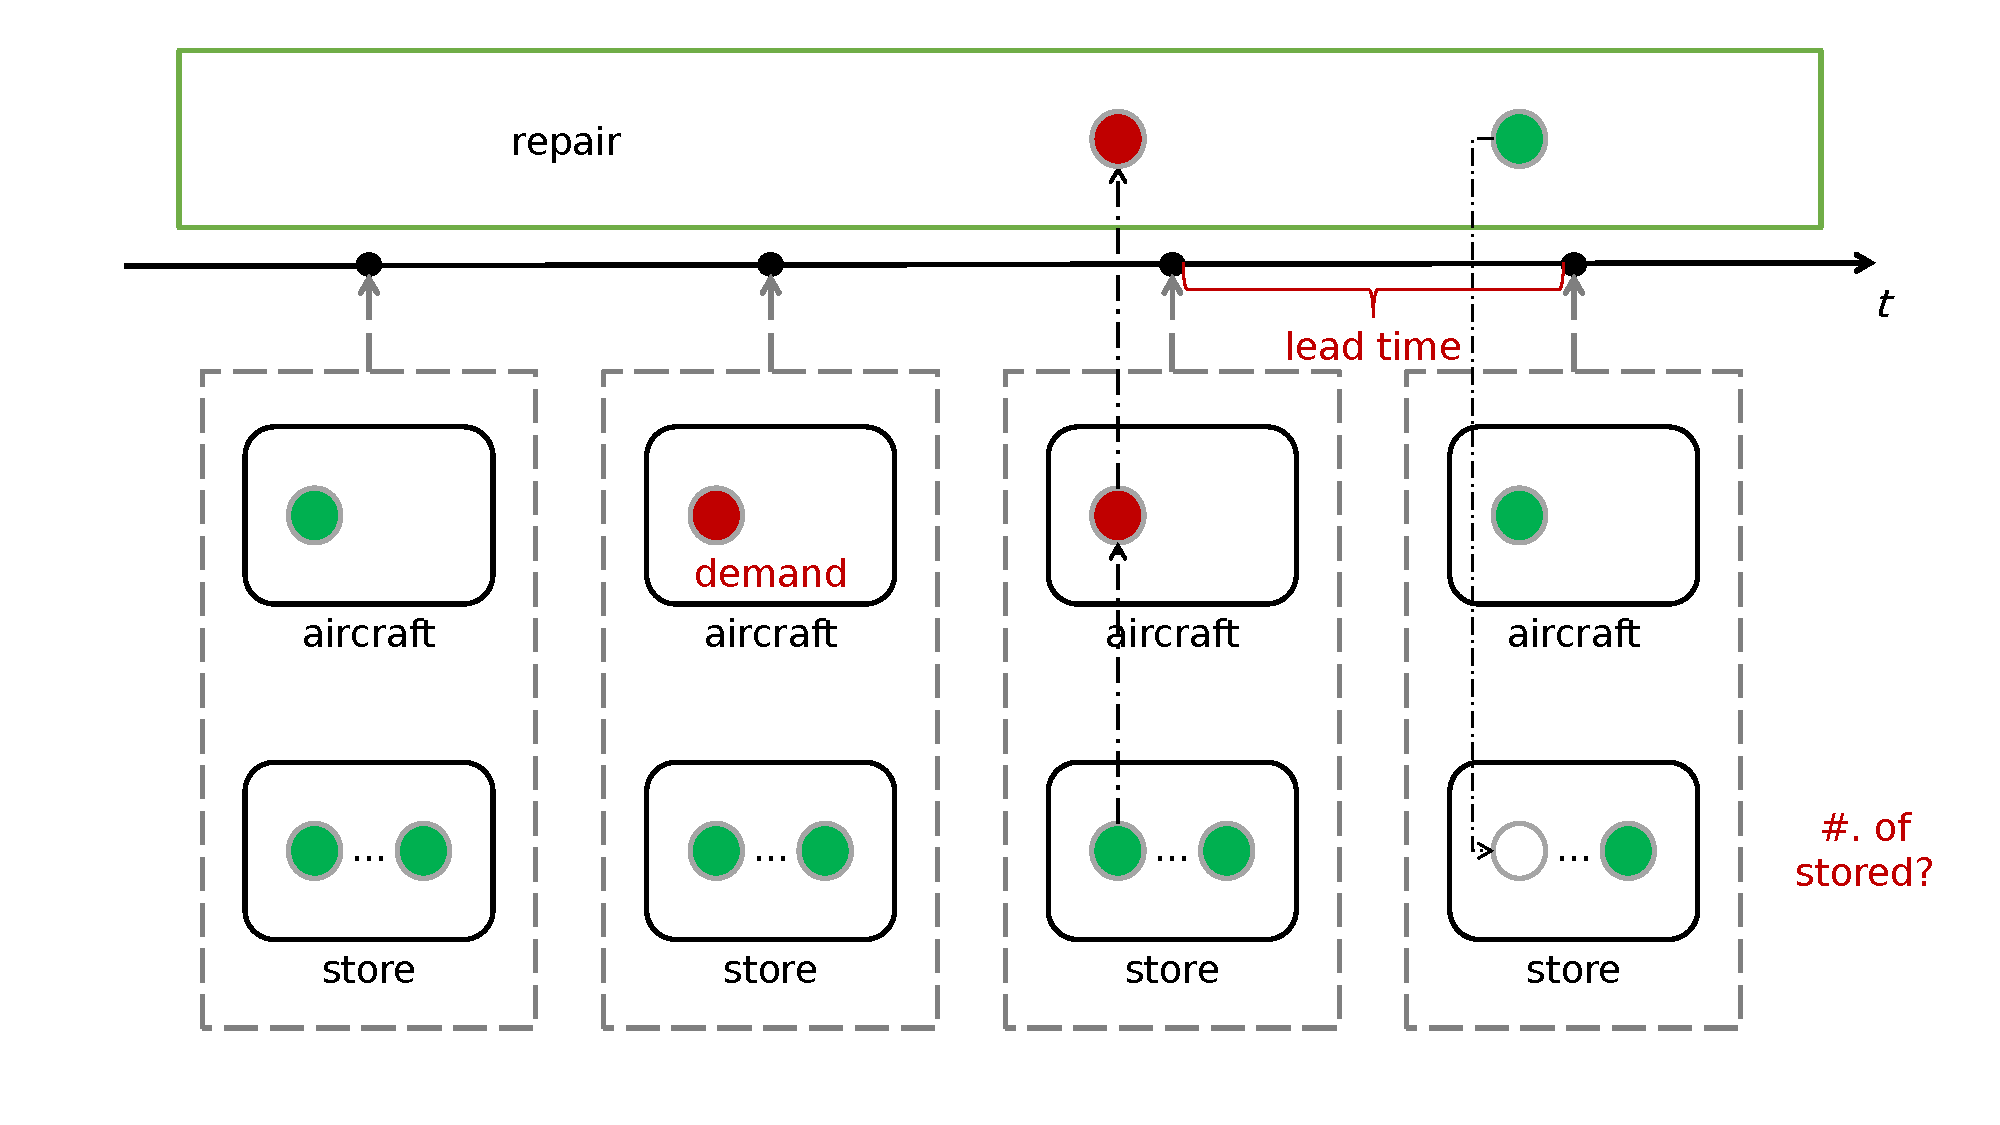
\includegraphics[width=11cm]{./images/rc2fig7.pdf}
\end{figure}


\end{frame}


\begin{frame}{Poisson, Gamma and Negative Binomial Distribution}

\structb{Application (continued).} We have the following models.
\begin{itemize}
	\justifying
	\item The demand is a random variable $R$ that follows a Poisson distribution
	\begin{align*}
	f_R(r|t) = \frac{e^{-\lambda t}(\lambda t)^r}{\Gamma(r + 1)},
	\end{align*}
	where $\lambda$ is the average number of demands per unit time, and $t$ denotes the lead time.
	\item The lead time $t$ follows a gamma distribution
	\begin{align*}
	f_T(t) = \frac{\mu e^{-\mu t} (\mu t)^{k-1}}{\Gamma(k)}, \qquad k > 0,
	\end{align*}
	which can be seen from $\alpha = k, \beta = \mu$.
\end{itemize}


\end{frame}

\begin{frame}{Poisson, Gamma and Negative Binomial Distribution}

\justifying
\structb{Application (continued).} Then the probability of $r$ demands during the lead time with parameter $k$ is
\begin{align*}
p_{rk} & = \int_0^{\infty} f_R(r|t) f_T(t) \U{d}t \qquad \red{(\U{recall\ } P[A] = \sum P[A|B]P[B])} \\
& = \int_0^{\infty} \frac{e^{-\lambda t}(\lambda t)^r}{\Gamma(r+1)} \times \frac{\mu e^{-\mu t}(\mu t)^{k-1}}{\Gamma(k)} \U{d}t \\
& = \frac{\lambda^t \mu^k}{\Gamma(r+1)\Gamma(k)}\int_0^{\infty} t^{r+k-1}e^{-(\lambda+\mu)t}\U{d}t \qquad \red{(\U{let\ }z = (\lambda + \mu)t)} \\
& = \frac{\lambda^r\mu^k}{(\lambda+\mu)^{r+k}\Gamma(r+1)\Gamma(k)}\int_0^{\infty} z^{r+k-1}e^{-z}\U{dz} \\
& = \frac{\lambda^r\mu^k}{(\lambda+\mu)^{r+k}}\times \frac{\Gamma(r+k)}{\Gamma(r+1)\Gamma(k)} = \binom{r+k-1}{k-1}\frac{(\lambda/\mu)^r}{(1+\lambda/\mu)^{r+k}},
\end{align*}
implying $r$ follows a negative binomial distribution with mean $\lambda k/\mu$ and variance $\lambda k/\mu(1+\lambda/\mu)$.


\end{frame}


\begin{frame}{Poisson, Gamma and Negative Binomial Distribution}

\justifying
\structb{Application (continued).} Next steps are basically the following.
\begin{enumerate}
	\justifying
	\item Calculate \emph{risk level} $P_{nk}$, defined by
	\begin{align*}
	P_{nk} = \sum_{r=n+1}^{\infty} p_{rk}.
	\end{align*}
	\item Predetermine the risk level, calculate the corresponding float size $n$.
\end{enumerate}
For more information, please see the file uploaded on canvas.

\end{frame}


\section{Exercises}

\subsection{Common Distributions}

\begin{frame}{Exercises}

\justifying
\structb{Exercise 1.} Suppose that a certain system contains three components $C_1, C_2, C_3$ that function independently of each other and are connected as series, so that the system fails as soon as one of the components fails. Suppose that the length of life of the $C_1, C_2, C_3$ has the exponential distribution with parameters
\begin{align*}
\beta_1 = 0.001, \qquad \beta_2 = 0.003, \qquad \beta_3 = 0.006,
\end{align*}
respectively, all measured in hours. Determine the probability that the system will not fail before 100 hours.

\end{frame}


\begin{frame}{Exercises}

\justifying
\structb{Exercise 2.} Let $X_1, X_2, X_3$ be independent lifetimes of memory chips. Suppose each $X_i$ follows the normal distribution with mean 300 hours and standard deviation 10 hours. Compute the probability that at least one of the three chips lasts at least 290 hours.

\end{frame}
